\section{Thực nghiệm}

\subsection{Bộ kiểm thử và môi trường}

\textbf{Bộ kiểm thử cố định} gồm 16 màn trong thư mục \texttt{Source/levels/}, chia thành 4 nhóm theo độ khó tăng dần, mỗi nhóm 4 màn (Hình 1). Mọi giải thuật chạy trên đúng cùng bộ màn này và mọi màn đều giải được (đã kiểm chứng bằng BFS).

{\renewcommand{\arraystretch}{1.25}
\begin{longtable}{|>{\raggedright\arraybackslash}p{0.098\linewidth}|>{\raggedright\arraybackslash}p{0.600\linewidth}|>{\raggedright\arraybackslash}p{0.196\linewidth}|}
\hline
\textbf{Nhóm} & \textbf{Đặc điểm} & \textbf{Màn} \\ \hline
\endhead
\hline
\endlastfoot
g1 & Cơ bản: chỉ có ô sàn thường, ô trống và ô đích & \texttt{g1\_\allowbreak{}basic\_\allowbreak{}01..04} \\ \hline
g2 & Có ô dễ vỡ (khối đứng lên sẽ rơi) & \texttt{g2\_\allowbreak{}fragile\_\allowbreak{}01..04} \\ \hline
g3 & Có công tắc và cầu (mềm, nặng, tách khối; đảo hoặc cố định trạng thái cầu) & \texttt{g3\_\allowbreak{}switch\_\allowbreak{}01..04} \\ \hline
g4 & Kết hợp ô dễ vỡ, công tắc, cầu và tách khối & \texttt{g4\_\allowbreak{}combined\_\allowbreak{}01..04} \\
\end{longtable}
}

\textbf{Môi trường chạy:} Intel Core i3-1115G4 @ 3,0 GHz (4 luồng), khoảng 8 GB RAM, Linux, Python 3.14.7.

Tổng cộng 16 màn × 5 giải thuật (BFS, DFS, IDS, UCS, A*) = 80 lượt chạy; \textbf{tất cả đều giải được}, không có lượt nào vượt giới hạn thời gian.

\subsection{Phương pháp đo hiệu năng}

Bốn chỉ số được ghi nhận cho mỗi lượt chạy, theo yêu cầu của đề bài:

{\renewcommand{\arraystretch}{1.25}
\begin{longtable}{|>{\raggedright\arraybackslash}p{0.229\linewidth}|>{\raggedright\arraybackslash}p{0.701\linewidth}|}
\hline
\textbf{Chỉ số} & \textbf{Cách đo} \\ \hline
\endhead
\hline
\endlastfoot
Thời gian tìm kiếm & \texttt{time.perf\_\allowbreak{}counter()} (đồng hồ độ phân giải cao, đơn điệu, không bị ảnh hưởng khi đổi giờ hệ thống) \\ \hline
Bộ nhớ đỉnh & \texttt{tracemalloc}, trừ đi mức bộ nhớ đã cấp phát lúc bắt đầu tìm kiếm để không tính phần chuẩn bị trước đó \\ \hline
Số nút mở rộng & Theo định nghĩa ở mục 4.1, đếm qua \texttt{MetricsTracker.count\_\allowbreak{}expansion()} \\ \hline
Độ dài lời giải & Số hành động của đường đi trả về \\
\end{longtable}
}

Ngoài ra, mỗi lời giải còn được gán một giá trị \textbf{cost} bằng tổng \texttt{physics\_\allowbreak{}cost} của đường đi, tính chung một thang cho mọi giải thuật để so sánh được cả với UCS và A*.

Ba biện pháp đảm bảo độ tin cậy của phép đo (Sơ đồ 7):

\begin{enumerate}
\item \textbf{Mỗi lần đo chạy trong một tiến trình con riêng} với giới hạn thời gian (mặc định 30 giây). Cách này dùng được trên mọi hệ điều hành (không phụ thuộc \texttt{SIGALRM}) và tiến trình bị dừng hẳn khi quá hạn.
\item \textbf{Thời gian và bộ nhớ được đo ở hai lần chạy riêng.} \texttt{tracemalloc} làm chậm chương trình khoảng 3 đến 4 lần nên thời gian được đo khi tắt nó; bộ nhớ đỉnh được đo ở một lần chạy bật nó.
\item \textbf{Các lượt chạy nhanh (dưới 1 giây) được lặp lại} (mặc định 3 lần) và lấy \textbf{trung vị}, vì màn nhỏ chạy chỉ vài mili giây nên một mẫu đơn lẻ chủ yếu là nhiễu.
\end{enumerate}

\begin{sodo}[!htbp]
\centering
\caption{Quy trình đo một cặp (màn, giải thuật)}
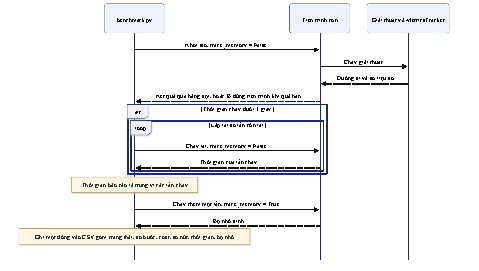
\includegraphics[width=0.95\linewidth,height=0.62\textheight,keepaspectratio]{images/sodo7.pdf}
\end{sodo}

\subsection{Quan sát trực quan cách các giải thuật duyệt không gian}

Hình 4 đặt BFS, DFS và IDS cạnh nhau trên cùng một màn nhỏ (g1\_basic\_03). Màu của mỗi ô cho biết thời điểm ô đó lần đầu bị một trạng thái được mở rộng chiếm giữ (vàng là sớm, tím là muộn); đường đen là lời giải được trả về.

\begin{figure}[!htbp]
\centering
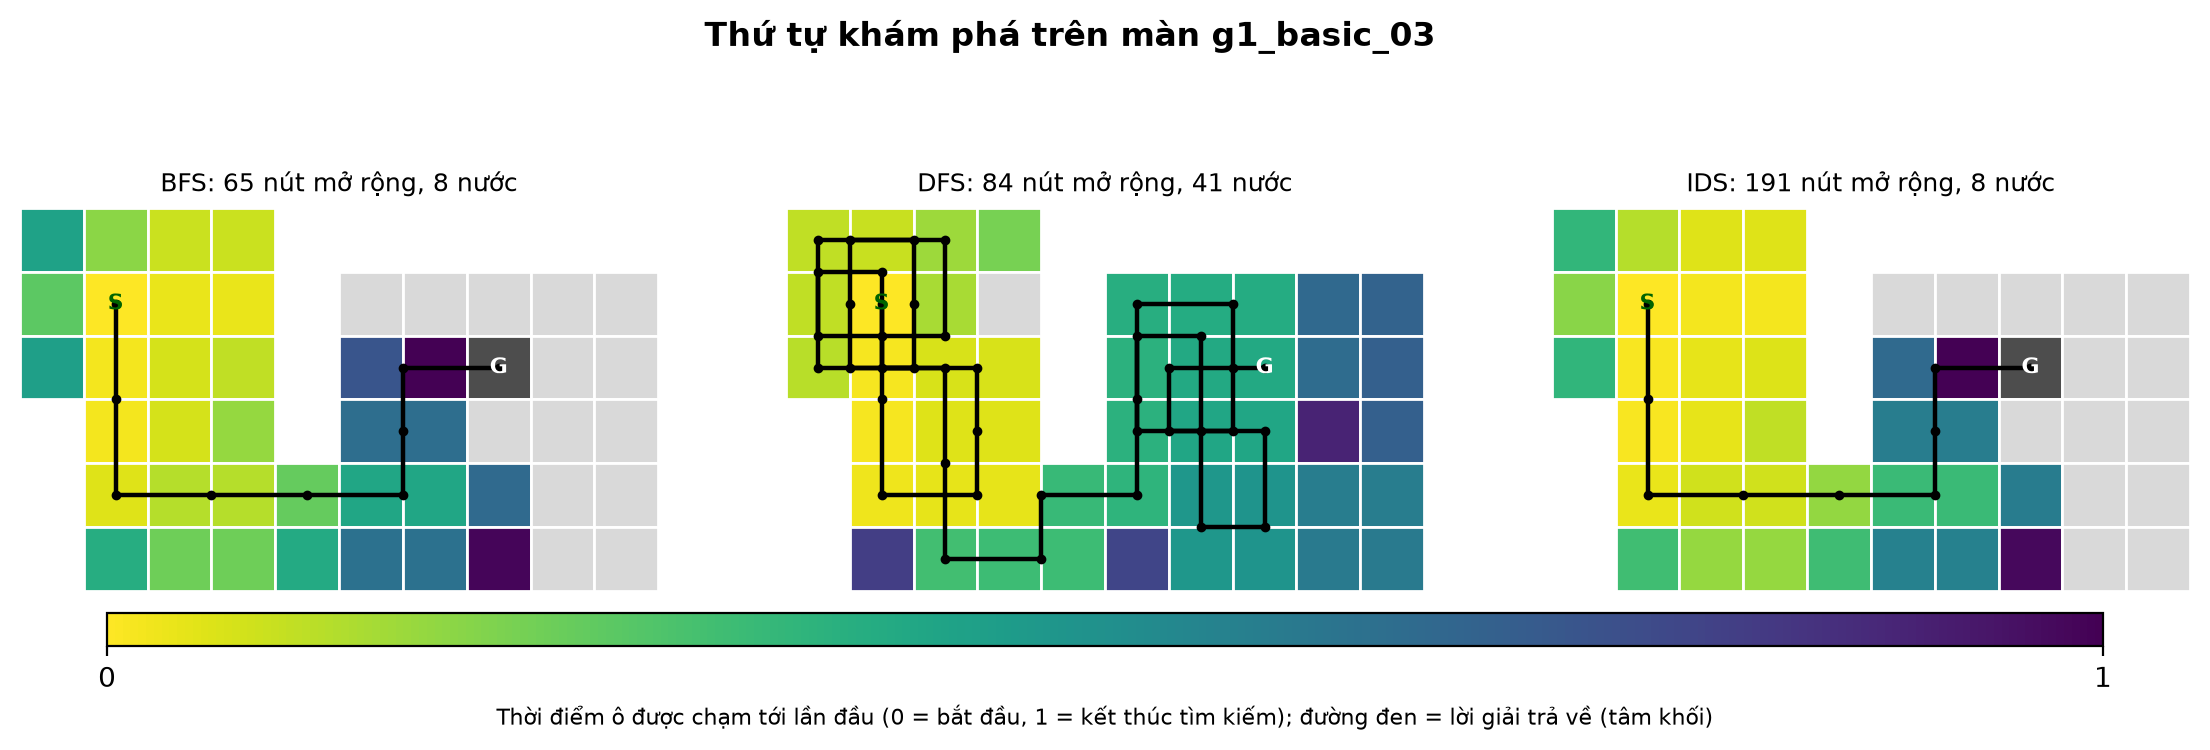
\includegraphics[width=\linewidth,height=0.45\textheight,keepaspectratio]{images/fig_exploration_order.png}
\caption{Thứ tự khám phá bàn chơi và lời giải của BFS (65 nút, 8 nước), DFS (84 nút, 41 nước) và IDS (191 nút, 8 nước) trên màn g1\_basic\_03.}
\end{figure}

Các quan sát từ hình:

\begin{itemize}
\item \textbf{BFS} lan đều theo mọi hướng từ ô xuất phát như một vết loang, nên màu chuyển dần từ vàng sang tím theo khoảng cách đến ô xuất phát, và đường đi ngắn gọn.
\item \textbf{DFS} đi sâu vào một vùng rồi quay lui. Phần bên trái của bàn bị đi đi lại lại nhiều lần trước khi sang được phía bên phải, dẫn tới lời giải 41 nước, dài hơn 5 lần lời giải tối ưu. Số nút mở rộng (84) còn lớn hơn BFS (65) trên màn này.
\item \textbf{IDS} cho cùng lời giải với BFS nhưng phải mở rộng 191 nút, gấp khoảng 3 lần BFS, do các lượt lặp.
\end{itemize}

\subsection{Bảng số liệu tổng hợp theo nhóm}

Các giá trị là \textbf{trung bình nhân} trên 4 màn của mỗi nhóm. Trung bình nhân được chọn vì số nút mở rộng trải qua nhiều bậc độ lớn giữa các màn; trung bình cộng sẽ bị một màn khó nhất (\texttt{g4\_\allowbreak{}combined\_\allowbreak{}04}) chi phối. UCS và A* được đưa vào để đối chiếu.

{\small\renewcommand{\arraystretch}{1.25}
\begin{longtable}{|l|l|r|r|r|r|r|}
\hline
\textbf{Nhóm} & \textbf{\makecell{Giải\\ thuật}} & \textbf{\makecell{Số\\ bước}} & \textbf{Cost} & \textbf{\makecell{Số nút\\ mở rộng}} & \textbf{\makecell{Thời gian\\ (ms)}} & \textbf{\makecell{Bộ nhớ\\ đỉnh (KB)}} \\ \hline
\endhead
\hline
\endlastfoot
g1 & BFS & 11,0 & 17,7 & 49 & 1,23 & 13,5 \\ \hline
g1 & DFS & 24,7 & 39,2 & 46 & 1,10 & 17,0 \\ \hline
g1 & IDS & 11,0 & 17,7 & 252 & 5,02 & 16,2 \\ \hline
g1 & UCS & 11,3 & 17,3 & 56 & 1,69 & 17,5 \\ \hline
g1 & A* & 11,3 & 17,3 & 46 & 1,58 & 16,0 \\ \hline
g2 & BFS & 21,6 & 33,8 & 78 & 1,85 & 21,4 \\ \hline
g2 & DFS & 30,9 & 48,9 & 53 & 1,31 & 19,7 \\ \hline
g2 & IDS & 21,6 & 33,8 & 1.501 & 26,15 & 29,6 \\ \hline
g2 & UCS & 22,0 & 33,4 & 83 & 1,98 & 27,5 \\ \hline
g2 & A* & 22,0 & 33,4 & 78 & 1,84 & 26,1 \\ \hline
g3 & BFS & 18,5 & 33,1 & 199 & 4,09 & 60,1 \\ \hline
g3 & DFS & 70,1 & 116,4 & 178 & 3,38 & 71,5 \\ \hline
g3 & IDS & 18,5 & 33,1 & 2.833 & 51,19 & 85,5 \\ \hline
g3 & UCS & 18,6 & 32,9 & 239 & 4,70 & 86,1 \\ \hline
g3 & A* & 18,6 & 32,9 & 198 & 4,34 & 75,1 \\ \hline
g4 & BFS & 22,8 & 33,6 & 2.836 & 46,79 & 942,3 \\ \hline
g4 & DFS & 114,5 & 162,7 & 171 & 3,61 & 98,8 \\ \hline
g4 & IDS & 22,8 & 33,6 & 48.008 & 819,42 & 1.398,7 \\ \hline
g4 & UCS & 22,8 & 33,6 & 5.290 & 99,74 & 1.866,8 \\ \hline
g4 & A* & 22,8 & 33,6 & 3.041 & 55,85 & 1.273,1 \\
\end{longtable}
}

Bảng chi tiết nhóm khó nhất (g4), nơi các giải thuật phân biệt rõ nhất:

{\small\renewcommand{\arraystretch}{1.25}
\begin{longtable}{|l|l|r|r|r|r|r|}
\hline
\textbf{Màn} & \textbf{\makecell{Giải\\ thuật}} & \textbf{\makecell{Số\\ bước}} & \textbf{Cost} & \textbf{\makecell{Số nút\\ mở rộng}} & \textbf{\makecell{Thời gian\\ (ms)}} & \textbf{\makecell{Bộ nhớ\\ đỉnh (KB)}} \\ \hline
\endhead
\hline
\endlastfoot
g4\_combined\_01 & BFS & 12 & 22 & 242 & 3,88 & 108,0 \\ \hline
g4\_combined\_01 & DFS & 24 & 42 & 42 & 0,96 & 16,6 \\ \hline
g4\_combined\_01 & IDS & 12 & 22 & 1.175 & 19,48 & 135,4 \\ \hline
g4\_combined\_02 & BFS & 29 & 39 & 4.597 & 74,68 & 1.233,2 \\ \hline
g4\_combined\_02 & DFS & 304 & 376 & 390 & 9,11 & 273,8 \\ \hline
g4\_combined\_02 & IDS & 29 & 39 & 104.403 & 1.906,44 & 1.949,9 \\ \hline
g4\_combined\_03 & BFS & 25 & 33 & 5.228 & 96,73 & 1.719,6 \\ \hline
g4\_combined\_03 & DFS & 141 & 181 & 224 & 5,21 & 147,4 \\ \hline
g4\_combined\_03 & IDS & 25 & 33 & 100.085 & 1.745,56 & 2.652,8 \\ \hline
g4\_combined\_04 & BFS & 31 & 45 & 11.118 & 171,15 & 3.444,0 \\ \hline
g4\_combined\_04 & DFS & 167 & 245 & 234 & 3,75 & 142,6 \\ \hline
g4\_combined\_04 & IDS & 31 & 45 & 432.630 & 6.954,95 & 5.465,3 \\
\end{longtable}
}

Bảng đầy đủ cho cả 16 màn và 5 giải thuật được đưa vào Phụ lục A.

\begin{figure}[!htbp]
\centering
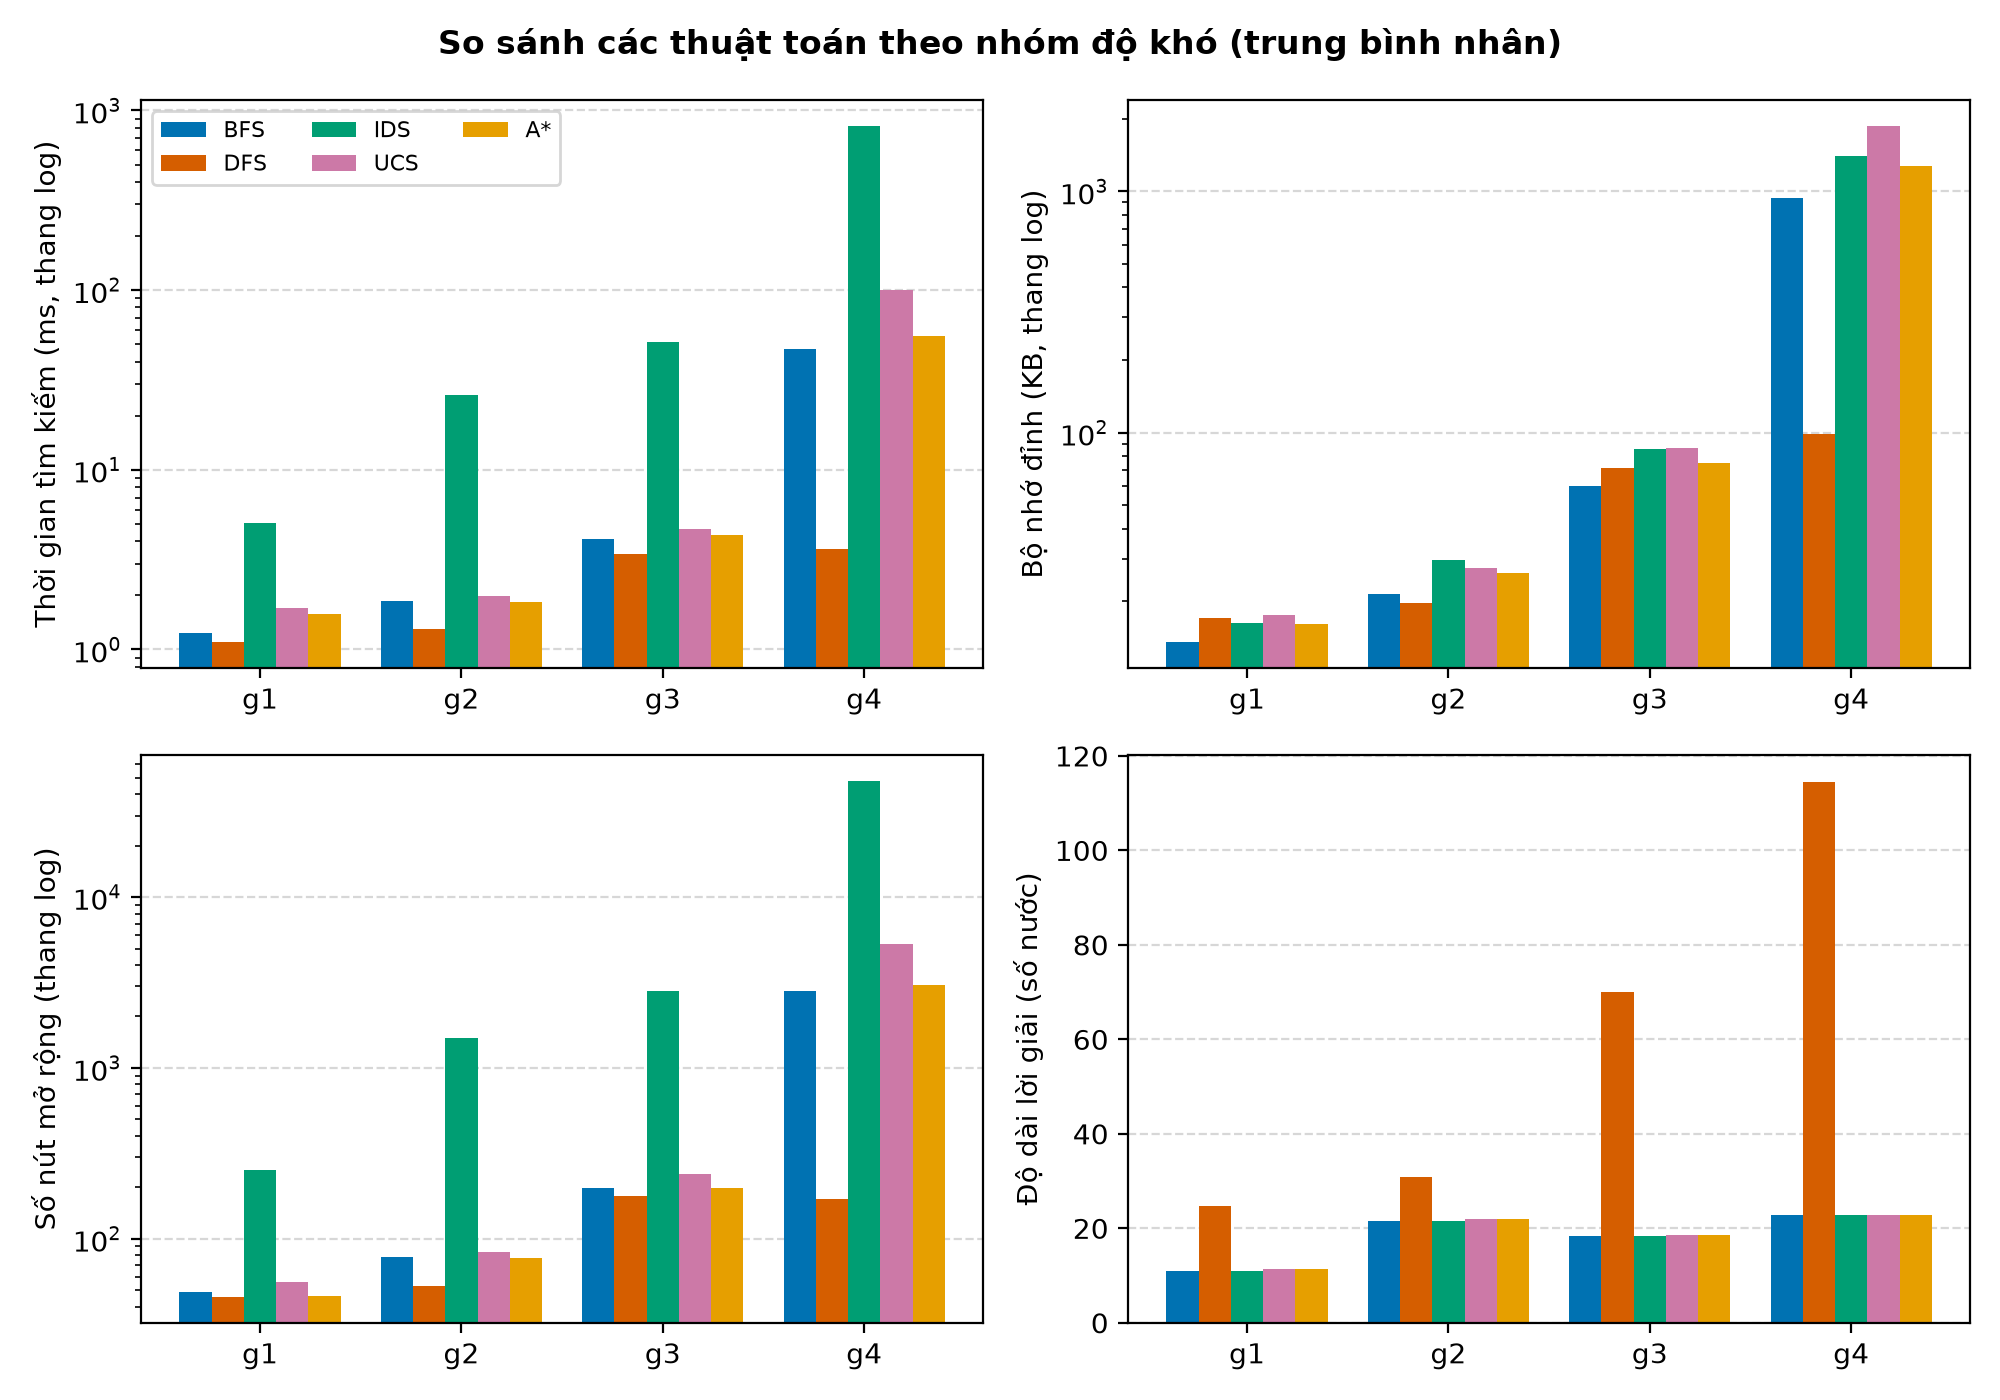
\includegraphics[width=\linewidth,height=0.45\textheight,keepaspectratio]{images/fig_metrics_by_group.png}
\caption{Thời gian, bộ nhớ, số nút mở rộng (thang log) và độ dài lời giải theo nhóm màn (trung bình nhân).}
\end{figure}

\begin{figure}[!htbp]
\centering
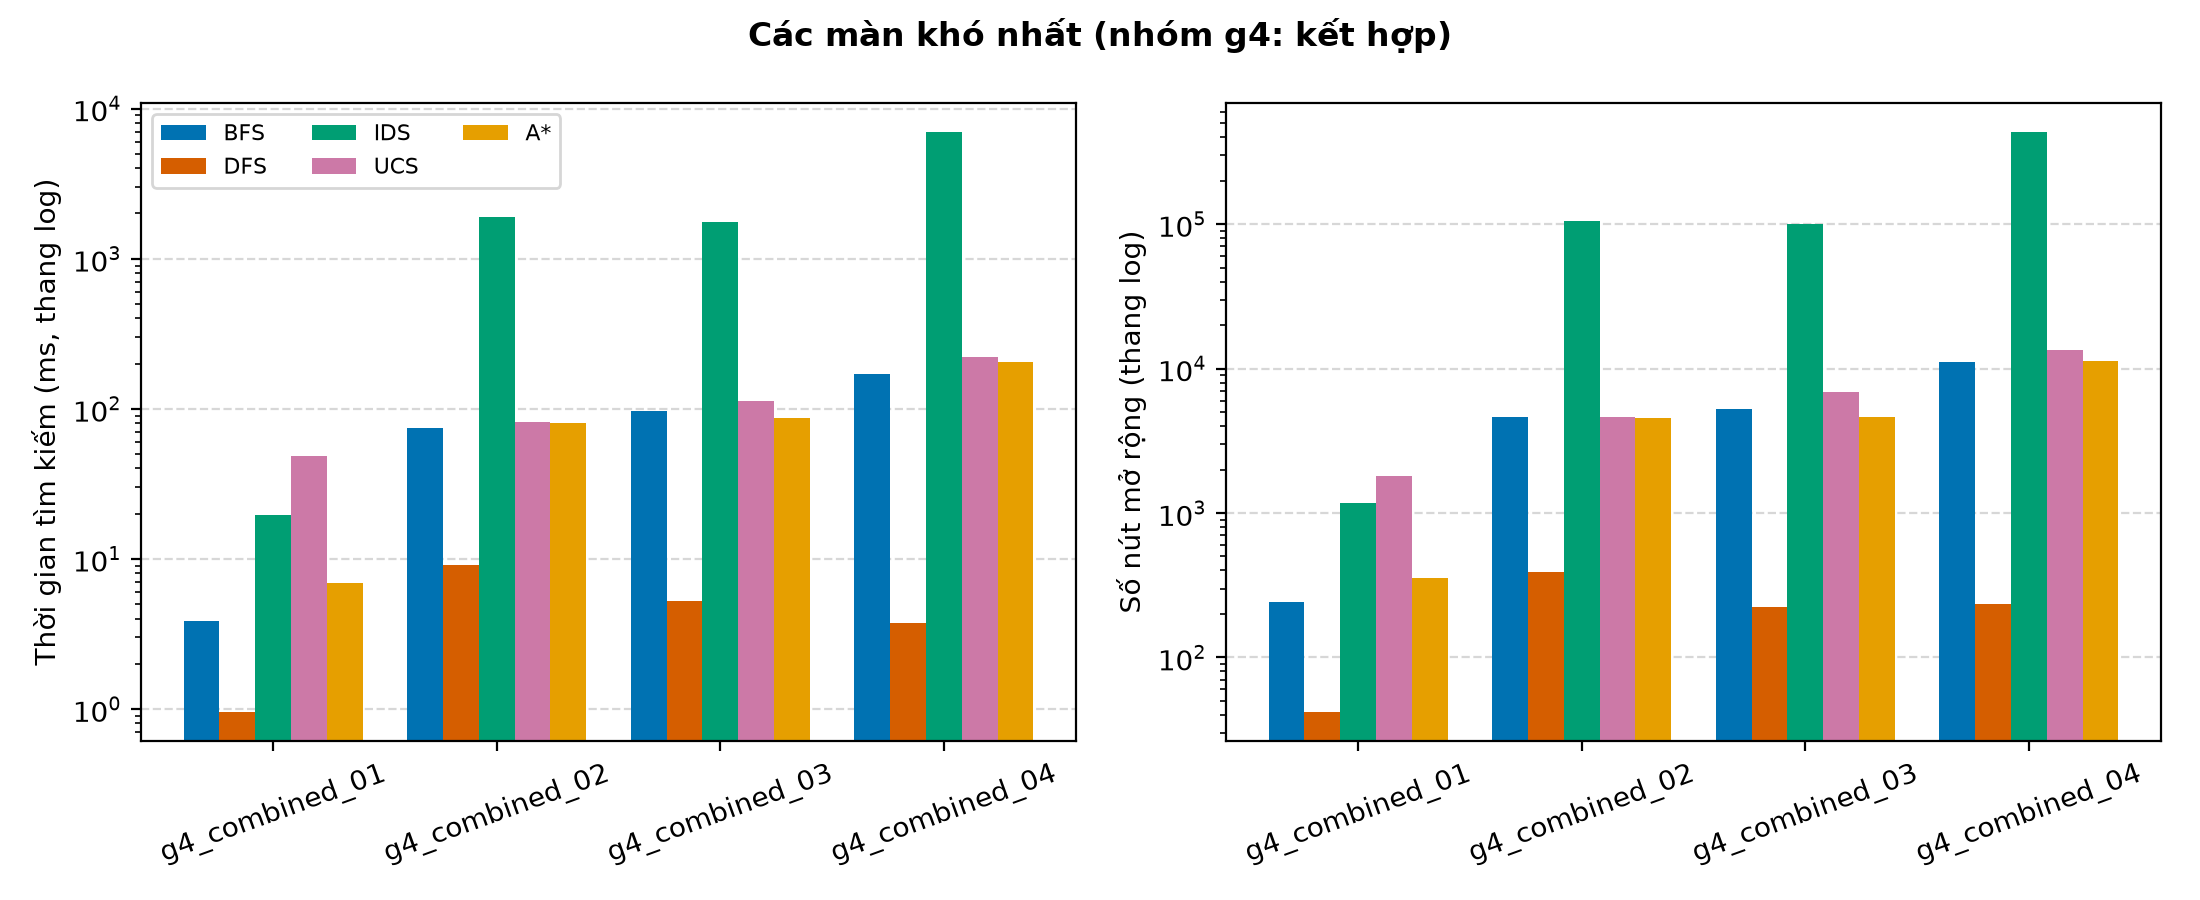
\includegraphics[width=\linewidth,height=0.45\textheight,keepaspectratio]{images/fig_hardest_levels.png}
\caption{Thời gian và số nút mở rộng trên 4 màn khó nhất (nhóm g4), thang log.}
\end{figure}

\subsection{Nhận xét}

\textbf{Chất lượng lời giải.}

\begin{itemize}
\item BFS và IDS cho \textbf{đúng cùng số bước ở cả 16 màn}, và đó là số bước nhỏ nhất, phù hợp với phần chứng minh ở mục 4.2.6 và 4.4.6.
\item Số bước nhỏ nhất \textbf{chưa chắc là cost nhỏ nhất}. Ở 3/16 màn, UCS và A* tìm được lời giải có cost thấp hơn dù nhiều bước hơn: \texttt{g1\_\allowbreak{}basic\_\allowbreak{}03} (BFS 8 bước, cost 14; UCS 9 bước, cost 13), \texttt{g2\_\allowbreak{}fragile\_\allowbreak{}01} (16 bước, cost 24; so với 17 bước, cost 23) và \texttt{g3\_\allowbreak{}switch\_\allowbreak{}04} (23 bước, cost 41; so với 24 bước, cost 40). Mức vượt trung bình chỉ 0,6 đến 1,9\% ở g1–g3 và 0\% ở g4 (Hình 7). Hai thước đo ``số nước đi'' và \texttt{physics\_\allowbreak{}cost} trùng nhau ở hầu hết các màn nhưng không phải luôn luôn, nên BFS và IDS tối ưu theo số nước đi mà không đảm bảo tối ưu theo cost.
\item DFS là giải thuật duy nhất cho lời giải \textbf{kém hẳn}: dài gấp 1,0 đến 10,5 lần lời giải ngắn nhất (trung vị khoảng 3,1 lần) và chỉ đạt cost tối ưu ở 1/16 màn (\texttt{g2\_\allowbreak{}fragile\_\allowbreak{}02}). Ở g4 lời giải trung bình là 114,5 nước so với 22,8 nước, cost cao hơn khoảng 384\%. Màn tệ nhất là \texttt{g4\_\allowbreak{}combined\_\allowbreak{}02}: 304 nước so với 29 nước tối ưu.
\end{itemize}

\begin{figure}[!htbp]
\centering
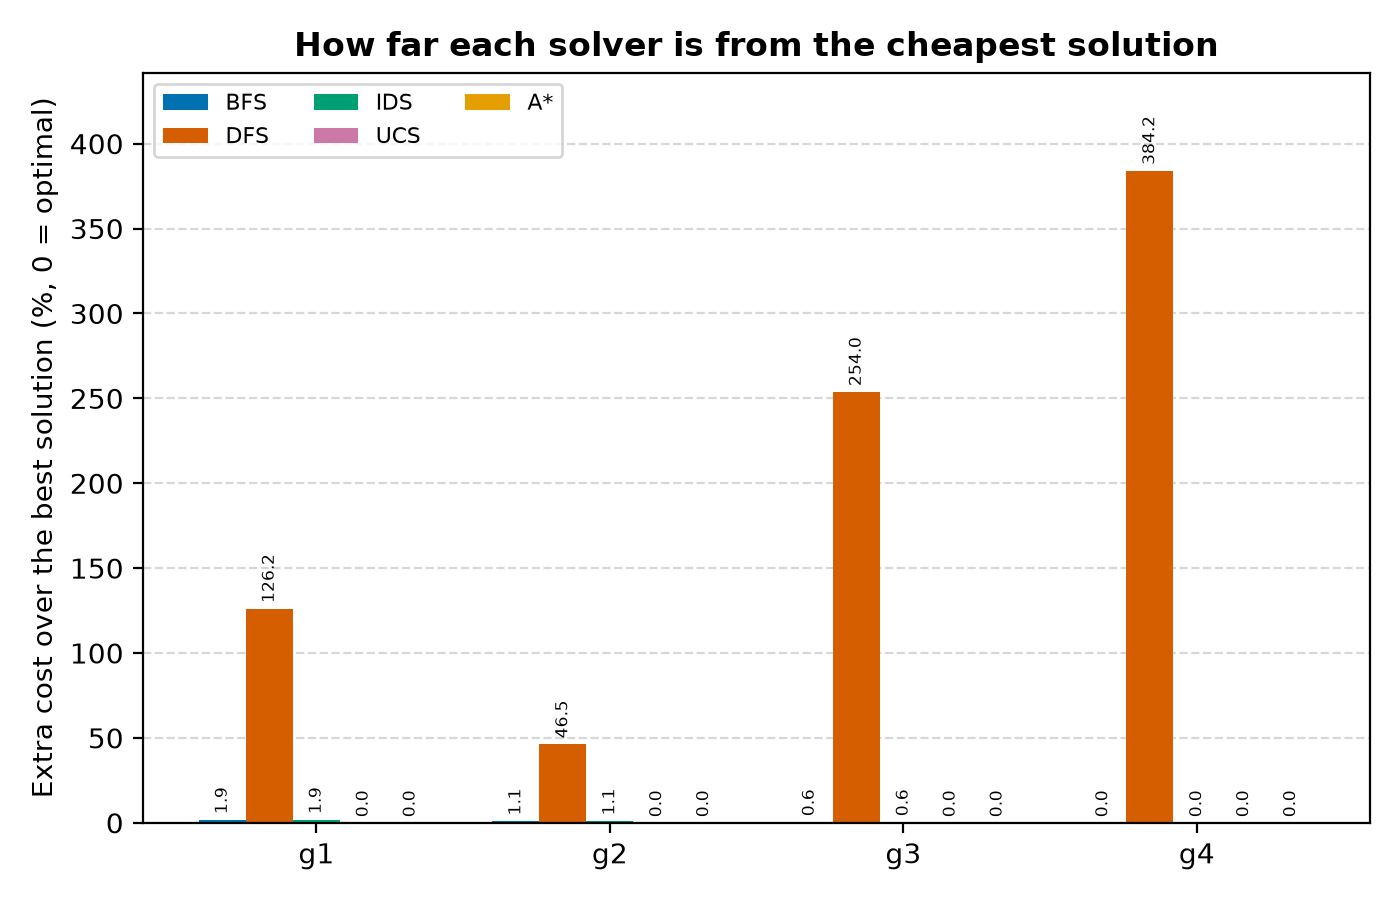
\includegraphics[width=\linewidth,height=0.45\textheight,keepaspectratio]{images/fig_cost_ratio.png}
\caption{Phần trăm cost vượt so với cost thấp nhất tìm được trên mỗi màn (0 nghĩa là tối ưu theo \texttt{physics\_\allowbreak{}cost}).}
\end{figure}

\textbf{Chi phí tìm kiếm.}

\begin{itemize}
\item \textbf{DFS} mở rộng ít nút hơn BFS ở 12/16 màn và nhanh nhất ở nhóm g4 (3,6 ms so với 46,8 ms của BFS), vì nó đi thẳng theo một nhánh mà không phải duyệt hết từng lớp. Đổi lại lời giải rất dài, và kết quả phụ thuộc vào thứ tự hành động cố định U, D, L, R: đổi thứ tự có thể cho kết quả khác hẳn. Ưu thế về tốc độ của DFS vì vậy mang tính may rủi chứ không phải được đảm bảo; Hình 4 cho thấy trên màn g1\_basic\_03 DFS thậm chí mở rộng nhiều nút hơn BFS.
\item \textbf{BFS} có số nút mở rộng tăng nhanh theo độ khó (49 nút ở g1 lên 2.836 nút ở g4, tăng khoảng 58 lần), vì số trạng thái tăng mạnh khi có thêm ô đặc biệt, cầu (mỗi cầu làm số cấu hình cầu có thể tăng tới gấp đôi) và khối tách.
\item \textbf{IDS} tốn kém nhất: mở rộng nhiều hơn BFS từ \textbf{2,9 đến 38,9 lần} và chậm hơn từ 2,6 đến 40,6 lần. Ở \texttt{g4\_\allowbreak{}combined\_\allowbreak{}04} IDS mở rộng 432.630 nút (so với 11.118 nút của BFS) và mất khoảng 7 giây. Nguyên nhân là mỗi lượt lặp mở rộng lại toàn bộ các trạng thái ở độ sâu nhỏ hơn (Hình 3); chênh lệch càng lớn khi lời giải càng sâu.
\end{itemize}

\textbf{Bộ nhớ.}

\begin{itemize}
\item Nhận định thường gặp ``DFS và IDS tốn ít bộ nhớ hơn BFS'' chỉ đúng với tìm kiếm dạng cây. Ở đây cả ba là tìm kiếm trên đồ thị nên đều phải giữ bảng các trạng thái đã thăm, và kết quả đo cho thấy:
\begin{itemize}
\item \textbf{IDS dùng nhiều bộ nhớ hơn BFS ở cả 16 màn} (gấp 1,2 đến 1,6 lần) do bảng \texttt{reached} và \texttt{parent} cộng thêm ngăn xếp.
\item \textbf{DFS dùng ít bộ nhớ hơn BFS ở 7/16 màn}, trong đó có cả 4 màn g4 (98,8 KB so với 942,3 KB). Nhưng ở nhiều màn nhỏ DFS dùng \emph{nhiều hơn} BFS (như \texttt{g1\_\allowbreak{}basic\_\allowbreak{}03}: 39,0 KB so với 20,3 KB), vì DFS đưa tất cả nút con vào ngăn xếp và \texttt{visited} trước khi quyết định đi tiếp. Ở g4 DFS tiết kiệm bộ nhớ chủ yếu vì nó tìm thấy đích chỉ sau khoảng 170 lần mở rộng, chứ không phải nhờ cấu trúc bộ nhớ tốt hơn.
\end{itemize}
\item Bộ nhớ của BFS tăng khoảng 70 lần từ g1 đến g4 (13,5 KB lên 942,3 KB), cùng xu hướng với số nút; DFS chỉ tăng khoảng 6 lần (17,0 KB lên 98,8 KB) vì số nút nó khám phá gần như không đổi.
\end{itemize}

\textbf{Theo nhóm độ khó.} Ở g1 và g2 (màn nhỏ), cả năm giải thuật đều chạy dưới 50 ms nên chênh lệch tuyệt đối không đáng kể dù IDS đã chậm hơn BFS hàng chục lần về tỉ lệ. Sự khác biệt về giá trị tuyệt đối chỉ lộ rõ ở g3 và nhất là g4, nơi công tắc, cầu và khối tách làm không gian trạng thái phình lên. Vì vậy các kết luận về hiệu năng nên chủ yếu dựa vào hai nhóm này.

\subsection{So sánh UCS và A*}

\subsubsection{So sánh số đỉnh mở rộng}

\textbf{Với \texttt{physics\_\allowbreak{}cost} ($c_{\text{stand}} = 3.0$):}

{\small\renewcommand{\arraystretch}{1.25}
\begin{longtable}{|l|r|r|r|r|r|}
\hline
\textbf{Màn} & \textbf{UCS (đỉnh mở)} & \textbf{A* (đỉnh mở)} & \textbf{Chi phí ($g^*$)} & \textbf{Bước} & \textbf{Giảm} \\ \hline
\endhead
\hline
\endlastfoot
g1\_basic\_01 & 44 & 37 & 12.0 & 8 & 15.9\% \\ \hline
g1\_basic\_02 & 61 & 56 & 20.0 & 12 & 8.2\% \\ \hline
g1\_basic\_03 & 89 & 60 & 13.0 & 9 & 32.6\% \\ \hline
g1\_basic\_04 & 40 & 37 & 29.0 & 19 & 7.5\% \\ \hline
g2\_fragile\_01 & 99 & 93 & 23.0 & 17 & 6.1\% \\ \hline
g2\_fragile\_02 & 49 & 43 & 31.0 & 19 & 12.2\% \\ \hline
g2\_fragile\_03 & 94 & 87 & 38.0 & 24 & 7.4\% \\ \hline
g2\_fragile\_04 & 106 & 104 & 46.0 & 30 & 1.9\% \\ \hline
g3\_switch\_01 & 203 & 187 & 29.0 & 15 & 7.9\% \\ \hline
g3\_switch\_02 & 130 & 95 & 24.0 & 14 & 26.9\% \\ \hline
g3\_switch\_03 & 374 & 309 & 42.0 & 24 & 17.4\% \\ \hline
g3\_switch\_04 & 333 & 281 & 40.0 & 24 & 15.6\% \\ \hline
g4\_combined\_01 & 1,816 & 357 & 22.0 & 12 & \textbf{80.3\%} \\ \hline
g4\_combined\_02 & 4,641 & 4,552 & 39.0 & 29 & 1.9\% \\ \hline
g4\_combined\_03 & 6,932 & 4,649 & 33.0 & 25 & 32.9\% \\ \hline
g4\_combined\_04 & 13,405 & 11,315 & 45.0 & 31 & 15.6\% \\ \hline
\textbf{Tổng cộng} & \textbf{28,416} & \textbf{22,262} & — & — & \textbf{21.7\%} \\
\end{longtable}
}

\emph{(Ghi chú: UCS và A* tìm ra kết quả đồng nhất cả về tổng chi phí tối ưu $g^*$ lẫn số bước đi trên mọi màn).}

\textbf{Với \texttt{unit\_\allowbreak{}cost} ($c_{\text{stand}} = 1.0$):}

{\small\renewcommand{\arraystretch}{1.25}
\begin{longtable}{|l|r|r|r|r|r|}
\hline
\textbf{Màn} & \textbf{UCS (đỉnh mở)} & \textbf{A* (đỉnh mở)} & \textbf{Chi phí ($g^*$)} & \textbf{Bước} & \textbf{Giảm} \\ \hline
\endhead
\hline
\endlastfoot
g1\_basic\_01 & 44 & 37 & 8.0 & 8 & 15.9\% \\ \hline
g1\_basic\_02 & 62 & 52 & 12.0 & 12 & 16.1\% \\ \hline
g1\_basic\_03 & 84 & 47 & 8.0 & 8 & \textbf{44.0\%} \\ \hline
g1\_basic\_04 & 40 & 40 & 19.0 & 19 & 0.0\% \\ \hline
g2\_fragile\_01 & 101 & 96 & 16.0 & 16 & 5.0\% \\ \hline
g2\_fragile\_02 & 45 & 41 & 19.0 & 19 & 8.9\% \\ \hline
g2\_fragile\_03 & 93 & 85 & 24.0 & 24 & 8.6\% \\ \hline
g2\_fragile\_04 & 105 & 104 & 30.0 & 30 & 1.0\% \\ \hline
g3\_switch\_01 & 180 & 121 & 15.0 & 15 & 32.8\% \\ \hline
g3\_switch\_02 & 125 & 72 & 14.0 & 14 & \textbf{42.4\%} \\ \hline
g3\_switch\_03 & 342 & 263 & 24.0 & 24 & 23.1\% \\ \hline
g3\_switch\_04 & 329 & 249 & 23.0 & 23 & 24.3\% \\ \hline
g4\_combined\_01 & 360 & 83 & 12.0 & 12 & \textbf{76.9\%} \\ \hline
g4\_combined\_02 & 4,627 & 3,594 & 29.0 & 29 & 22.3\% \\ \hline
g4\_combined\_03 & 5,544 & 3,822 & 25.0 & 25 & 31.1\% \\ \hline
g4\_combined\_04 & 11,563 & 8,129 & 31.0 & 31 & 29.7\% \\ \hline
\textbf{Tổng cộng} & \textbf{23,644} & \textbf{16,835} & — & — & \textbf{28.8\%} \\
\end{longtable}
}

\subsubsection{Nhận xét}

\begin{enumerate}
\item \textbf{Tính tối ưu tuyệt đối về chi phí:} Trên toàn bộ 16 màn, A* luôn tìm được lời giải có \textbf{cùng tổng chi phí tối ưu $g^*$} (và khớp hoàn toàn số bước) với UCS. Đây là hệ quả trực tiếp của tính admissible và consistent đã được chứng minh chặt chẽ cả trên lý thuyết lẫn qua kiểm chứng thực nghiệm 123,355 cạnh.
\item \textbf{Minh chứng thực nghiệm cho hiệu ứng của \texttt{physics\_\allowbreak{}cost}:} So sánh chéo giữa hai bảng thực nghiệm, tại 3 màn \texttt{g1\_\allowbreak{}basic\_\allowbreak{}03}, \texttt{g2\_\allowbreak{}fragile\_\allowbreak{}01} và \texttt{g3\_\allowbreak{}switch\_\allowbreak{}04}, số bước trong lời giải tối ưu của \texttt{physics\_\allowbreak{}cost} dài hơn \texttt{unit\_\allowbreak{}cost} đúng 1 bước:
\begin{itemize}
\item Ở \texttt{g1\_\allowbreak{}basic\_\allowbreak{}03}: \texttt{unit\_\allowbreak{}cost} đi 8 bước (tiêu tốn $14.0$ nếu quy đổi theo physics cost), trong khi \texttt{physics\_\allowbreak{}cost} đi 9 bước (chỉ tốn $13.0$).
\item Ở \texttt{g2\_\allowbreak{}fragile\_\allowbreak{}01}: \texttt{unit\_\allowbreak{}cost} đi 16 bước (tiêu tốn $24.0$ physics cost), trong khi \texttt{physics\_\allowbreak{}cost} đi 17 bước (chỉ tốn $23.0$).
\item Ở \texttt{g3\_\allowbreak{}switch\_\allowbreak{}04}: \texttt{unit\_\allowbreak{}cost} đi 23 bước (tiêu tốn $41.0$ physics cost), trong khi \texttt{physics\_\allowbreak{}cost} đi 24 bước (chỉ tốn $40.0$).
\end{itemize}
Thuật toán UCS và A* đã chủ động chọn đường lăn ngang dài hơn 1 bước nhằm triệt tiêu bớt một bước dựng đứng tốn kém (chi phí $3.0$). Minh chứng thực tế này khẳng định hàm \texttt{physics\_\allowbreak{}cost} đã thay đổi hành vi tìm kiếm theo đúng mô hình tối ưu năng lượng cơ học đã đề ra ở mục 5.1.4.
\item \textbf{Hiệu quả tìm kiếm:} A* giảm trung bình \textbf{21.7\%} số đỉnh mở rộng so với UCS trên \texttt{physics\_\allowbreak{}cost} và \textbf{28.8\%} trên \texttt{unit\_\allowbreak{}cost}. Heuristic phát huy hiệu quả mạnh nhất trên các màn có không gian trạng thái phức tạp và phân nhánh rộng:
\begin{itemize}
\item \texttt{g4\_\allowbreak{}combined\_\allowbreak{}01}: giảm tới \textbf{80.3\%} (physics) / \textbf{76.9\%} (unit) — heuristic cắt tỉa gần như toàn bộ các nhánh đi chệch hướng khỏi mục tiêu.
\item \texttt{g3\_\allowbreak{}switch\_\allowbreak{}02}: giảm \textbf{26.9\%} (physics) / \textbf{42.4\%} (unit) — heuristic dẫn hướng hiệu quả qua các cây cầu và công tắc.
\end{itemize}
\item \textbf{Trường hợp heuristic ít cải thiện:} Trên các màn có địa hình hành lang hẹp hoặc bắt buộc chỉ có một con đường hợp lệ duy nhất:
\begin{itemize}
\item \texttt{g2\_\allowbreak{}fragile\_\allowbreak{}04}: chỉ giảm 1.9\% (physics) — bản đồ dài và hẹp, hầu hết các trạng thái sinh ra đều thuộc về tuyến đường khả dĩ duy nhất.
\item \texttt{g1\_\allowbreak{}basic\_\allowbreak{}04}: giảm 0.0\% (unit) — không gian không có nhánh cụt dư thừa để cắt tỉa.
\end{itemize}
\end{enumerate}

\subsection{Ưu điểm và nhược điểm}

{\renewcommand{\arraystretch}{1.25}
\begin{longtable}{|>{\raggedright\arraybackslash}p{0.070\linewidth}|>{\raggedright\arraybackslash}p{0.263\linewidth}|>{\raggedright\arraybackslash}p{0.263\linewidth}|>{\raggedright\arraybackslash}p{0.263\linewidth}|}
\hline
 & \textbf{Ưu điểm} & \textbf{Nhược điểm} & \textbf{Phù hợp khi} \\ \hline
\endhead
\hline
\endlastfoot
\textbf{BFS} & Đảm bảo ít nước đi nhất; đơn giản; ổn định, ít phụ thuộc thứ tự hành động & Số nút và bộ nhớ tăng nhanh theo độ khó; không đảm bảo cost tối ưu khi chi phí không đồng nhất & Cần lời giải ngắn nhất và không gian trạng thái vừa phải \\ \hline
\textbf{DFS} & Nhanh và ít nút nhất ở màn khó; mã nguồn ngắn & Lời giải rất dài (tới 10 lần); kết quả phụ thuộc thứ tự hành động; không tối ưu & Chỉ cần một lời giải bất kỳ, càng nhanh càng tốt \\ \hline
\textbf{IDS} & Tối ưu số nước như BFS; kết luận được ``không giải được'' & Chậm nhất, mở rộng nhiều nút nhất vì lặp lại; trong cài đặt trên đồ thị không tiết kiệm bộ nhớ so với BFS & Khi cần tính tối ưu và hạn chế bộ nhớ chặt (dạng cây thuần túy) \\
\end{longtable}
}

Ưu điểm và nhược điểm của UCS và A*:

\textbf{UCS}

{\renewcommand{\arraystretch}{1.25}
\begin{longtable}{|>{\raggedright\arraybackslash}p{0.447\linewidth}|>{\raggedright\arraybackslash}p{0.483\linewidth}|}
\hline
\textbf{Ưu điểm} & \textbf{Nhược điểm} \\ \hline
\endhead
\hline
\endlastfoot
Đảm bảo tối ưu với mọi hàm chi phí dương. & Không có dẫn hướng, mở rộng đều theo mọi hướng (``tìm kiếm mù''). \\ \hline
Cài đặt đơn giản, không cần heuristic. & Mở nhiều đỉnh không cần thiết trên bản đồ lớn. \\ \hline
Hoạt động đúng ngay cả khi chi phí không đồng nhất. & Hiệu suất kém hơn A* khi có heuristic tốt. \\
\end{longtable}
}

\textbf{A*}

{\renewcommand{\arraystretch}{1.25}
\begin{longtable}{|>{\raggedright\arraybackslash}p{0.465\linewidth}|>{\raggedright\arraybackslash}p{0.465\linewidth}|}
\hline
\textbf{Ưu điểm} & \textbf{Nhược điểm} \\ \hline
\endhead
\hline
\endlastfoot
Giảm đáng kể số đỉnh mở rộng so với UCS (trung bình 21–29\%). & Cần thiết kế heuristic chặt chẽ: sai sẽ mất tính tối ưu. \\ \hline
Vẫn đảm bảo tính tối ưu nhờ heuristic admissible + consistent. & Heuristic dựa trên Manhattan distance nên ít hiệu quả trên bản đồ hẹp, dài, hoặc bản đồ có nhiều cầu (khoảng cách Manhattan bị biến dạng do cầu đóng/mở làm gián đoạn đường đi thực tế). \\ \hline
Heuristic consistent → không bao giờ re-open đỉnh → hiệu quả bộ nhớ. & Trên bản đồ nhỏ (\textless{} 100 đỉnh), chi phí tính heuristic có thể không bù được lợi ích cắt tỉa. \\ \hline
Trên bản đồ lớn (g4), tiết kiệm tới 80\% số đỉnh mở rộng. & Cần điều chỉnh tham số $c_{\text{stand}}$ theo hàm chi phí (đã tự động hóa). \\
\end{longtable}
}

\subsection{Hạn chế của thực nghiệm}

\begin{itemize}
\item Mỗi nhóm chỉ có 4 màn nên trung bình nhân chỉ có ý nghĩa định tính.
\item Thời gian là trung vị của 3 lần chạy trên một máy, có thể dao động theo tải hệ thống; các màn g1–g2 chạy chỉ vài mili giây nên sai số tương đối lớn. Bộ nhớ đo bằng \texttt{tracemalloc} chỉ tính phần cấp phát bởi Python, không phải toàn bộ RAM của tiến trình.
\item Kết quả của DFS gắn với thứ tự hành động cố định và không thể khái quát cho thứ tự khác.
\end{itemize}
